\documentclass[a4paper,11pt]{article}
\usepackage[a4paper,margin=1in,footskip=0.25in]{geometry}
\usepackage[utf8]{inputenc}
\usepackage{graphicx}
\usepackage{float}
\usepackage{parskip}
\usepackage[style=apa]{biblatex}
\addbibresource{exp.bib}
\usepackage{hyperref}


\title{What challenges are raised by the dissemination and/or communication of knowledge?}
\author{Terry Qi}

% TODO: 979 words need 950 max, proofread
% TODO: change search result to Douglass

\begin{document}

\maketitle

Word Count: 931

Objects:
\begin{enumerate}
 \item The law of demand within my economics book
 \item The bible according to Spike Milligan
 \item Google search result of Fredrick Douglass
\end{enumerate}

\newpage

% Uncertainty
% Context
% Oversaturation

% intro
% This exhibition will explore the prompt by reflecting upon the knowledge within the sciences, more specifically answering whether uncertainty hinder the acceptance and communication of knowledge. While mathematicians often take deductive proofs as granted, this is less common in the area of sciences. Every experiment contains empirical results, but depending on different people with their own personal backgrounds, beliefs, ideologies, or perspectives, the significance of the result will differ between the members of the public. More directly, the lack of trust in the sciences may be a disbelief towards its empirical methods, that uncertainty is untrustworthy and does not bring knowledge.


% knowable thing but could be failified
\subsection*{Object \ref{fig:lod}, The Law of Demand}

\begin{figure}[h!]
 \centering
 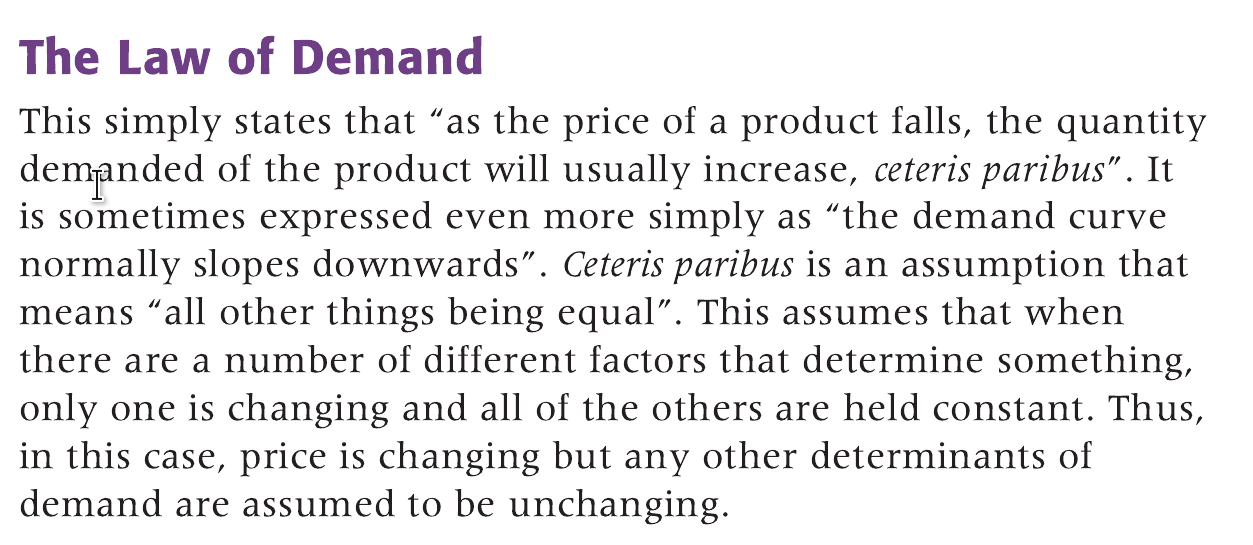
\includegraphics[scale=0.3]{ecobook.png}
 \caption{The law of demand as stated in the book}
 \label{fig:lod}
\end{figure}

This formula comes from my economics course book, and is widely controversial within our class for its inclusion of the word ``law'', for the formula is the historical avant-garde in a sense of certainty within the social sciences. Its idea is also attacked globally, particularly by psychologists arguing that the law is too idealistic in the context of real life, so much so that it divided economics into two branches \parencite{DKahneman}.

The formula is interesting for it is an expression of the scientists' bold beliefs in their models. Economists often back up the law through idealistic claims that are intentionally broad, marking its failures as a violation of the assumptions. This displays a case of false certainty --- making a relationship of human behavior to be more knowable than it truly is. On the one hand, it justifies many aspects of modern economic theories, with empirical evidence of its success reflected in economical growth numbers; but it also creates confusion for the learners and critics: coming from a maths background, I did not initially buy into the ``law'' for its vagueness. The framework allows economists to justify their actions while leaving its foundations deliberately broad, making the theory difficult to critique.

This object showcases the difficulties in the communication of theories with uncertain evidences.  While uncertainty is appealing as it eases the efforts needed to model human behavior; it is also difficult to be trusted for its assumptions. In my case, only after a discussion with the teacher and my further research on the topic did I feel comfortable applying its contents and the corollaries. Therefore the method of the distribution of knowledge serves to be significant. While dissemination techniques like speeches will reach a wider audience, they are relatively inefficient in conveying knowledge --- beliefs of information, then more direct methods like education and books. In the wider context, the disbeliefs in science is likely to be connected to the lack of proper communication.

% The natural scientists' critique only serves to reveal the flaws in their ``scientific methods'', that the entirety of physics is in essence, fitting numbers to interpretations. While both parties disagrees in acknowledging the shakiness of their disciplines, they are similar in framing the confusion as an ``interesting property'' and a benefit of the sciences, ultimately displaying how the interpretation of empirical evidence differs depending on your personal beliefs and backgrounds.

% context
\subsection*{Object \ref{fig:bible}, The bible according to Spike Milligan}

\begin{figure}[h!]
 \centering
 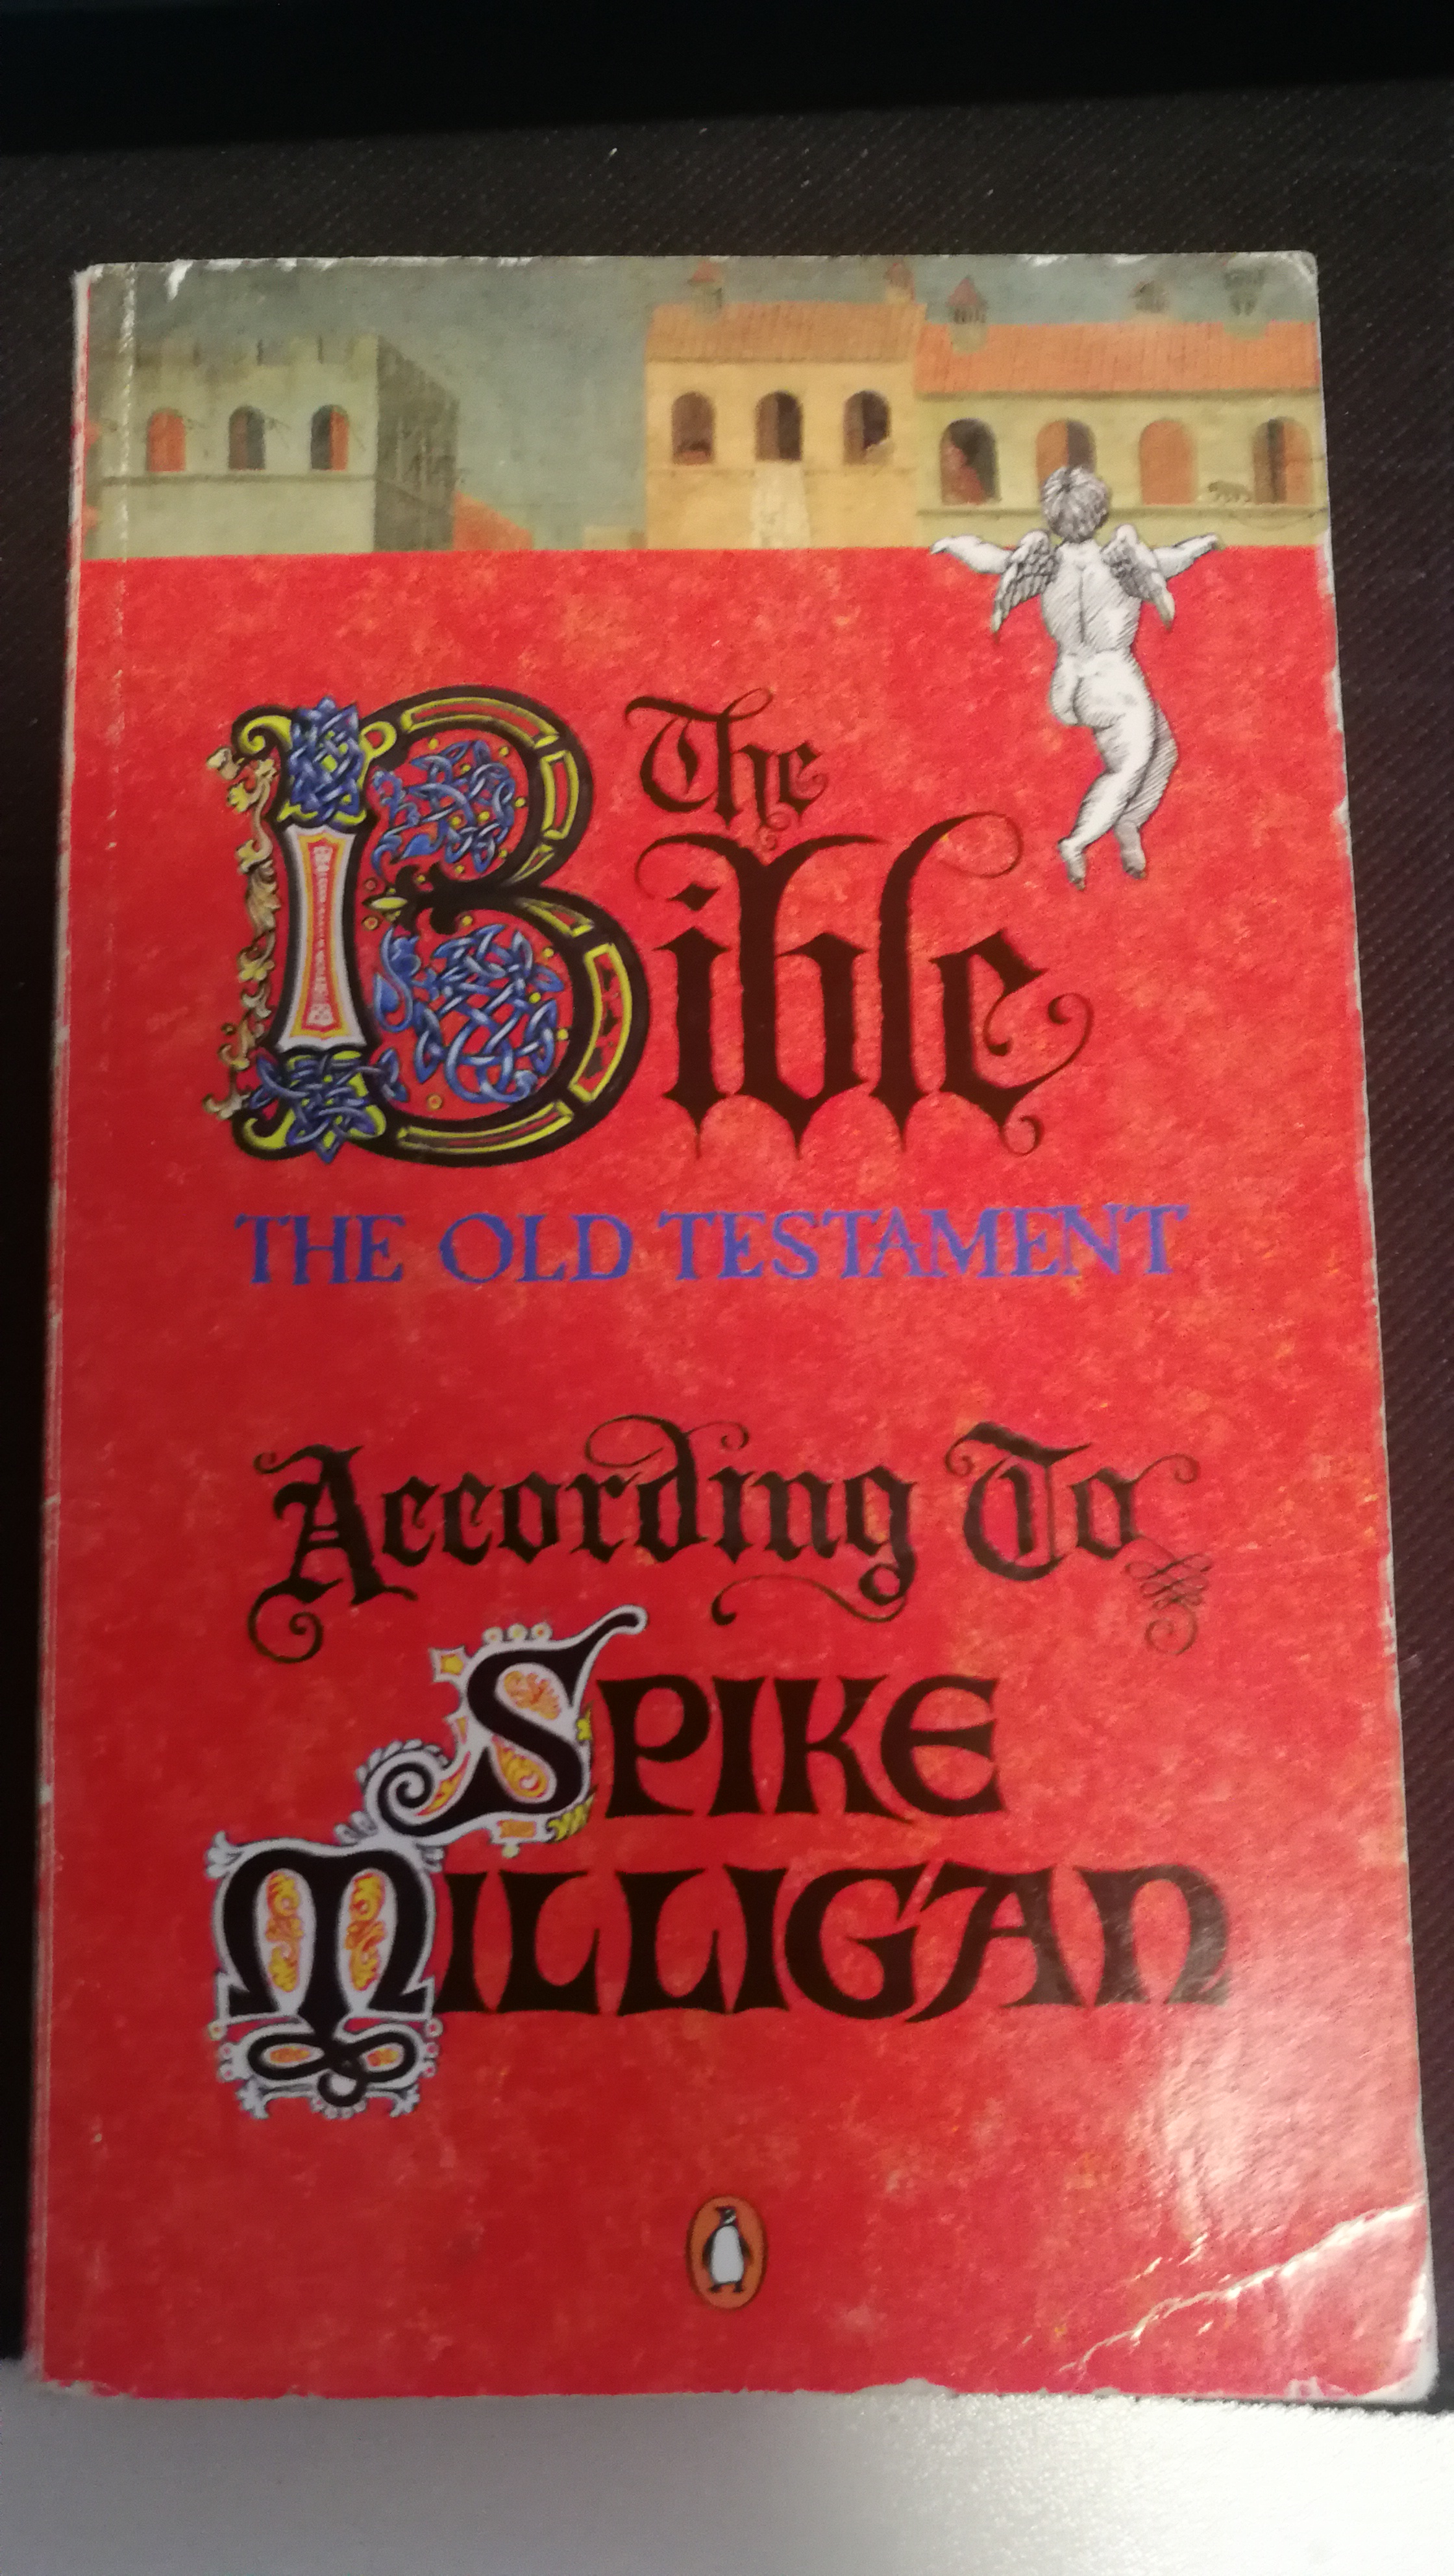
\includegraphics[scale=0.05]{bible.jpg}
 \caption{The bible according to Spike Milligan}
 \label{fig:bible}
\end{figure}

The object is a book issued to me by my history friend out of interest, for it parodies the old testament of the bible. The holy bible itself is interesting for its distinct context/origin is quite distinct --- people often disagree on the origin of the bible. Some, and I, use this fact to justify our disbeliefs of the knowledges within the bible. However, for Spike Milligan had only modified this context while retaining the knowledge the bible presents, it is interesting that I find myself enjoying its stories and tales.

My positive personal experience showcases how context can be challenging in the dissemination of knowledge. It is the uncertain origin of the book that breaks my interest, and respect towards the bible; but the interesting origin --- that of a British company, is what bring out my interest and respect towards Spike Milligan's parody. This showcase the importance of context in the communication of knowledge, for the parody received even positive reviews online from a mainly non-christian audience \parencite{Review}.

% When people think about the bible, they think of the connection and quotations within it rather than the plausibility and validity of the work. Historically speaking, the bible is special in its unknown origin and writer. Some people view this uncertainty as an argument to reject all meanings within the book, some accepts the knowledge it presents and not by its origin, and some values both interpretations equality.


%The parody of the bible is intriguing for it beautifully shows how the context of its origin can be completely different while retaining its messages and knowledge. The first chapter references the creation of the world, but from a perspective of a British startup firm. Unexpectedly, this shows that the messages of the bible --- that God is took seven days to create the world, is independent of its context, showcasing how the uncertainty of the origin can have little effects on the knowledge presented.

Therefore I included this parody of the bible in the exhibition to be an example where context helps the communication of knowledge. Furthermore, it displays the inevitability of biases in the form of context within the distribution the knowledge, for a single piece of work can be rephrased to appeal to a wider audience. This implies the possibility of knowledge to be distorted or even lost overtime --- a realistic example of a phenomenon of ``Chinese Whispers''.

% Judging from the positive reviews from the various purchasers and I, it seems to display the ability of a common ideology or pure interest to decrease the significance of the context of knowledge. This is in analogy to the ideas presented by the economists --- that the idealistic axioms are justified by a significant result in the knowledge that it creates.


% The object is my personal simulation of some swinging double pendulums. On the surface, it seems that the advances in the natural sciences should be able predict its motions to the atom. But the discovery of chaos questions the fundamental values of physics as a whole. In a sense, some people consider the possibility of uncertainty to be roadblock in the acquiring of knowledge in the sciences.

%Physics as a discipline follows a trend of experiment, theories, and prediction to formulate our understanding of the universe.

% unknowable thing that expresses certainty
\subsection*{Object \ref{fig:download}, Google search result of Fredrick Douglass}

\begin{figure}[h!]
 \centering
 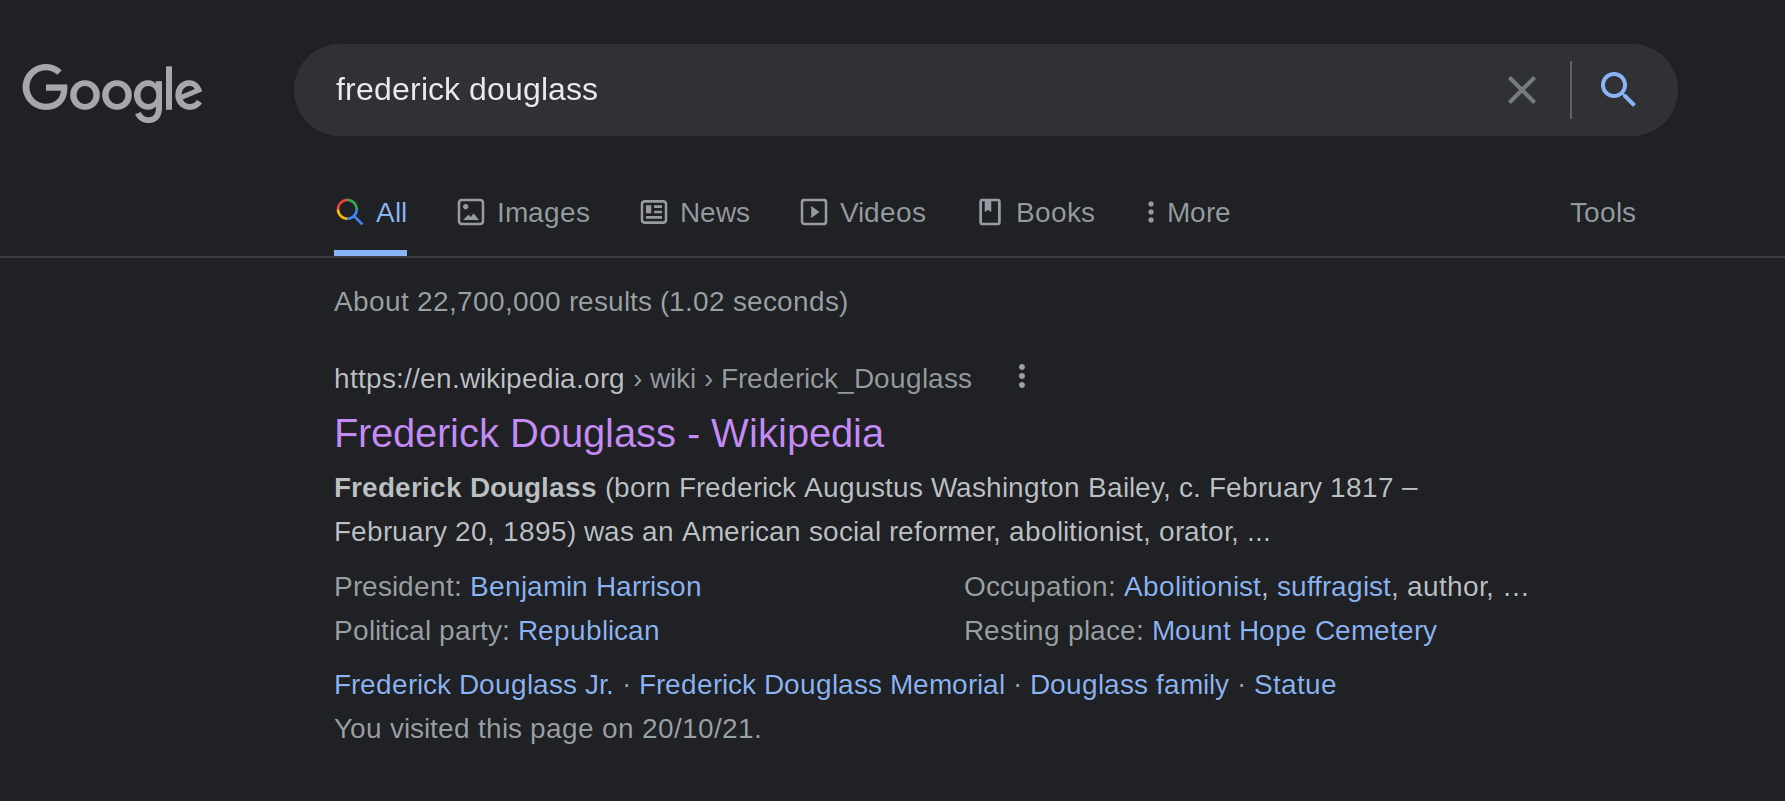
\includegraphics[scale=0.25]{douglass.png}
 \caption{Google search result of Fredrick Douglass}
 \label{fig:download}
\end{figure}

The object here is my personalized Google search result for person Fredrick Douglass. The invention of search engines and the internet had brought entire catalogues of encyclopedias to devices that you can hold in your hand. But the easiness of information can also be a challenge in the distribution of information, as one can be overwhelmed with billions of sources (shown in the object with 22 billion results). This often creates a heuristic bias favoring
easy information rather than correct information on the internet.

The website Wikipedia is a prime example of this oversaturation of knowledge. As seen in the object, the Wikipedia page is the first result out of the billion possible websites that relates to the query ``fredrick douglass'' --- and it is not a one-off. The top placement of Wikipedia results on Google search causes knowledge seekers to seek information on the website --- the Wikipedia page showing the life story of Fredrick Douglass.
The single source of information narrows the scope of human knowledge --- students often conduct research based on Wikipedia alone, and I have heavily relied on this page for my English research and didn't brother finding other perspectives on his life. This displays the difficulty in the communication of ideas online --- only popular websites are shown, and showcases the consequences of oversaturation during the dissemination and communication of knowledge online --- that people lose decision making abilities in their selection of information on the internet.

 %People in the 21st century would often pick the most visible and easiest route to get information and knowledge on a subject, creating a bias towards a single source of truth stemming from the effects of an oversaturation of knowledge.

The importance of the internet at the modern age justifies this object's position in my exhibition. Its statistics on the number of results made me realize the true difficulty in understanding a topic from all views on the internet, which poses a challenge for me to find all the perspectives on the speaker. Moreover, the sea of information on the internet may imply a future where knowledge does not exist, a world full of only opinions and persuasive writings due to the laziness and inability for humans to check all trillion sources on a single war, displaying the hypothetical peek of the challenges in the communication of truth. Sometimes in life, the less decisions the better, and the less information, the more meaningful they are.

%The object is a progress bar of a file download in the my Firefox browser. It have the purpose of displaying the time it takes to download this very important file I need. This sight had only became more common in the information era, yet it had surprised me to know that the underlying progress it displays has no certainty. The progress bar serves as a distraction to the nondeterministic information of file downloading for the user.

%While this little bar can come in many forms, there exist an endless flow of people complaining the inaccuracy of the device, yet the purpose of the device is for good --- to create feedback upon an action. It implies the idea that covering uncertainty with certainty, where knowledge is deliberately hidden, is undesirable to people. Additionally, versions of progress bars which does not cover the uncertainty does not escape the criticisms. It seems to me that people fear the concept of covering uncertainty with certainty, showcasing inability to reduce uncertainty in the communication of knowledge.

%The common appearances (and criticisms it faces) of the item helps in broadening the scope of the knowledge question. The progress bar showcases the general knower's desire for information in the event of a knowledge barrier, and its fear for the censoring of knowledge. For I have made progress bars myself in my apps, I find the understanding of the underlying knowledge the bar covers --- whether uncertain or not, helps in reducing the frustration of such a progress bar. This showcases the ability of uncertainty, even if covered with certainty, to induce frustration and communication of knowledge.

\nocite{*}
\printbibliography


\end{document}
